\documentclass[a4paper,12pt]{article}
\usepackage{amsmath}% http://ctan.org/pkg/amsmath
\usepackage{amssymb}
\usepackage{amsthm}
\usepackage{mdframed}
\usepackage{mathtools}
\usepackage{listings}% http://ctan.org/pkg/listings
\usepackage{enumitem}
\usepackage{import}
\usepackage{xifthen}
\usepackage{pdfpages}
\usepackage{transparent}
\usepackage{float}
\usepackage{hyperref}
\usepackage{booktabs}
\usepackage{pdfpages}
\newtheorem{theorem}{Theorem}[section]
\newtheorem{corollary}{Corollary}[theorem]
\newtheorem{lemma}[theorem]{Lemma}
\newtheorem*{remark}{Remark}
\newtheorem{definition}{Definition}[section]
\newenvironment{ftheorem}
  {\begin{mdframed}\begin{theorem}}
  {\end{theorem}\end{mdframed}}
\newenvironment{fcorollary}
  {\begin{mdframed}\begin{corollary}}
  {\end{corollary}\end{mdframed}}
\newenvironment{flemma}
  {\begin{mdframed}\begin{lemma}}
  {\end{lemma}\end{mdframed}}
\newenvironment{fremark}
  {\begin{mdframed}\begin{remark}}
  {\end{remark}\end{mdframed}}
\newenvironment{fdefinition}
  {\begin{mdframed}\begin{definition}}
  {\end{definition}\end{mdframed}}

\hypersetup{
    colorlinks=true,
    linkcolor=blue,
    filecolor=magenta,      
    urlcolor=cyan,
    pdftitle={Overleaf Example},
    pdfpagemode=FullScreen,
    }
\urlstyle{same}
\newcommand{\incfig}[1]{%
    \def\svgwidth{\columnwidth}
    \import{./Figures/}{#1.pdf_tex}
}

\title{Matlab Project \#73 report}
\date{\today}
\author{Long Nguyen}

\begin{document}
\maketitle

\section{Project requirements}

Build a function \verb|fun| that takes as input two vectors \verb|u| and \verb|v|
and as output provides the vector \verb|w| which contains in each entry
the max between the same entry position of the two vectors.

Download 2 audio signals and load them into Matlab.
Use the function \verb|fun| applied to the first 0.3 seconds of the
\textbf{first audio channel} of the 2 signals.
Plot the original 2 audio signals and the one obtained using the
function in a single figure using subplots.

Generate a report in pdf containing the results obtained,
including all the codes created.

\section{Results}

\subsection*{Main function}
\lstinputlisting[language=Matlab]{main.m}

\subsection*{Function output}
\begin{verbatim}
  "File Name: "    "clair-de-lune"    ".mp3"

  Number of Channels: 2
  Sample Rate: 44100
  Duration: 0.30002 seconds
      "File Name: "    "moonlight-sonata"    ".mp3"
  
  Number of Channels: 2
  Sample Rate: 48000
  Duration: 0.30002 seconds
\end{verbatim}

\subsection*{Output graphs}

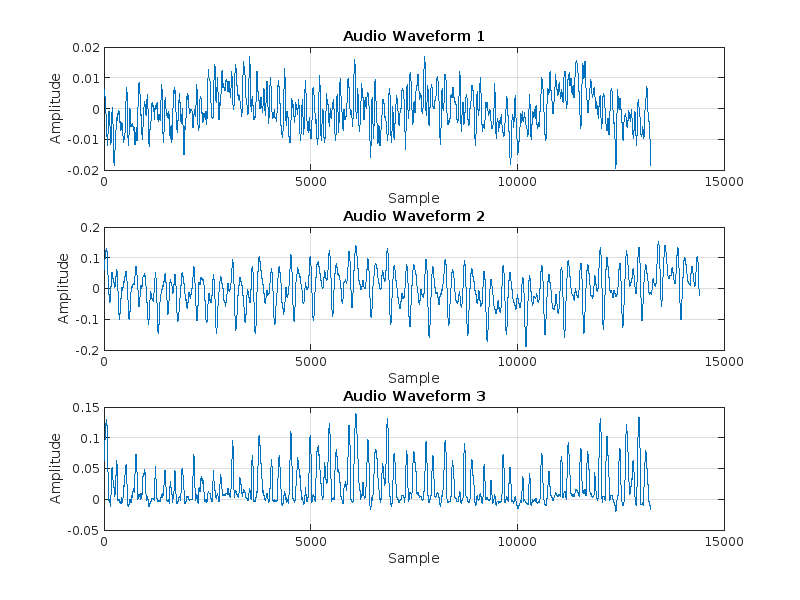
\includegraphics[width=\textwidth]{rendered/audio_result_no_normalize.png}

\section{Extra funcitonalities}

\subsection{Function read\_audio}

This function has the following extra functionalities:
\begin{itemize}
  \item The start and stop time to process the audio can be adjusted. In the main file, I am getting data from second 33 till 33.3 of both audio files.
  \item The last parameter is for audio normalization if specified as true.
\end{itemize}

\subsubsection*{Ouput of the function if normalization is set to true}
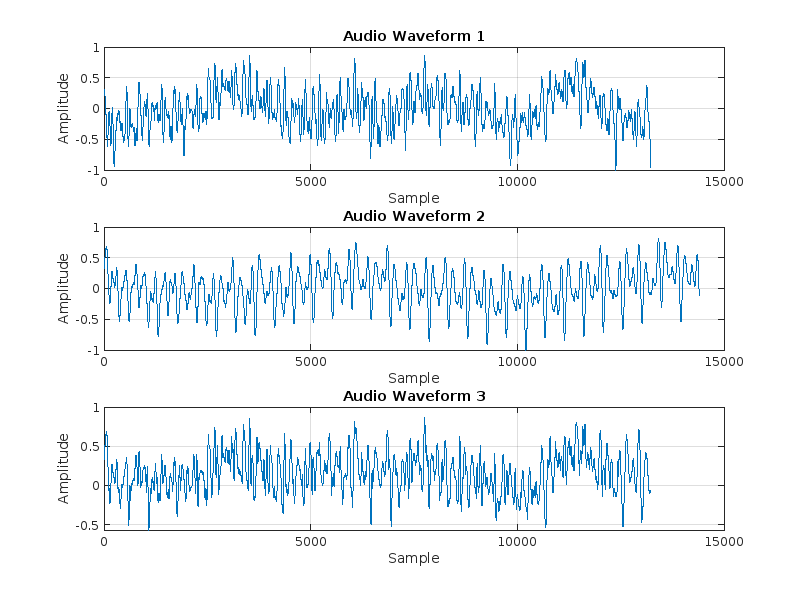
\includegraphics[width=\textwidth]{rendered/audio_result_normalized.png}

And when zoomed in:

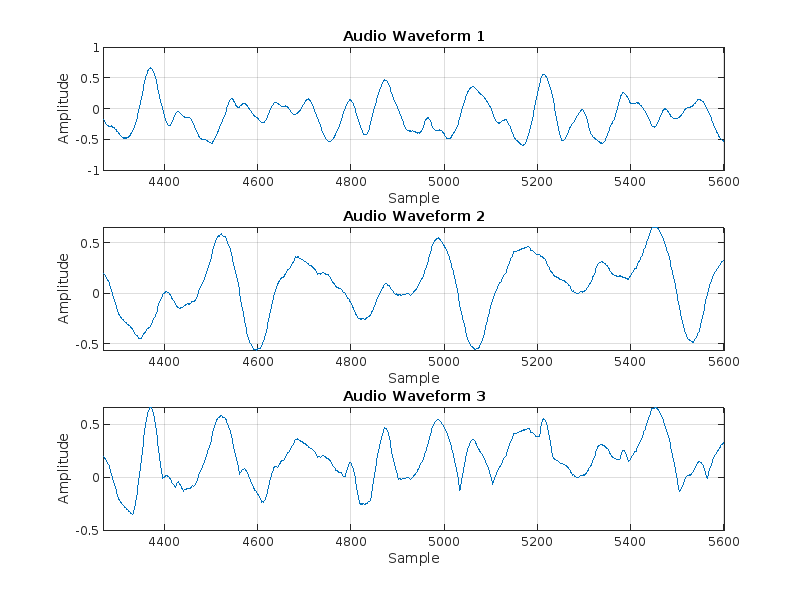
\includegraphics[width=0.95\textwidth]{rendered/audio_result_normalized_zoomed.png}

\subsection{Source control}

Soucre control is enabled for this project and it is located at

https://github.com/longieee/univaq-intro-to-matlab-final-project

\subsection{Unit tests}

Unit tests are also written for the functions of this project. The unit test code is located inside the \verb|tests| folder.

\subsection{Github workflow}

A simple Github workflow is also created for this project. The workflow is located at \verb|.github/workflows/matlab_test.yml|
and it is triggered on every push to the main branch to automatically run the unit tests.

A possible real-life application: The workflow runs the unit tests and if they pass, it will create a new release with the version number incremented by 1.

\section{Listing of all source code}

\subsection*{Folder structure}
\begin{verbatim}
  .
  |____LICENSE
  |____tests
  | |____test_read_audio.m
  | |____test_audio_plot.m
  | |____test_extendVectors.m
  | |____test_fun.m
  |____utils
  | |____fun.m
  | |____read_audio.m
  | |____extendVectors.m
  | |____audio_plot.m
  |____report.synctex.gz
  |____README.md
  |____report.tex
  |____rendered
  | |____audio_result_no_normalize.png
  | |____audio_result_normalized.png
  | |____project-description.pdf
  | |____audio_result_normalized_zoomed.png
  |____.gitignore
  |____main.m
  |____static
  | |____moonlight-sonata.mp3
  | |____clair-de-lune.mp3
  |____.github
  | |____workflows
  | | |____matlab_tests.yml
  |____report.pdf
\end{verbatim}

\subsection*{Main file (main.m)}
\lstinputlisting[language=Matlab]{main.m}

\pagebreak
\subsection*{Utilitiy functions}

\subsubsection*{Function fun}
\lstinputlisting[language=Matlab]{utils/fun.m}
\subsubsection*{Function read\_audio}
\lstinputlisting[language=Matlab]{utils/read_audio.m}
\subsubsection*{Function extendVectors}
\lstinputlisting[language=Matlab]{utils/extendVectors.m}
\subsubsection*{Function audio\_plot}
\lstinputlisting[language=Matlab]{utils/audio_plot.m}

\pagebreak
\subsection*{Unit tests}
\subsubsection*{Unit test for fun}
\lstinputlisting[language=Matlab]{tests/test_fun.m}
\subsubsection*{Unit test for read\_audio}
\lstinputlisting[language=Matlab]{tests/test_read_audio.m}
\subsubsection*{Unit test for extendVectors}
\lstinputlisting[language=Matlab]{tests/test_extendVectors.m}
\subsubsection*{Unit test for audio\_plot}
\lstinputlisting[language=Matlab]{tests/test_audio_plot.m}

\pagebreak
\subsection*{Other files}
\subsubsection*{Github workflow}
\lstinputlisting{.github/workflows/matlab_tests.yml}

\end{document}